\documentclass[tikz]{standalone}

\usepackage{fontspec}

\usetikzlibrary{arrows}
\usetikzlibrary{calc}
\usetikzlibrary{decorations.pathreplacing}
\usetikzlibrary{positioning}
\usetikzlibrary{matrix}

\usepackage{fontspec}

\begin{document}

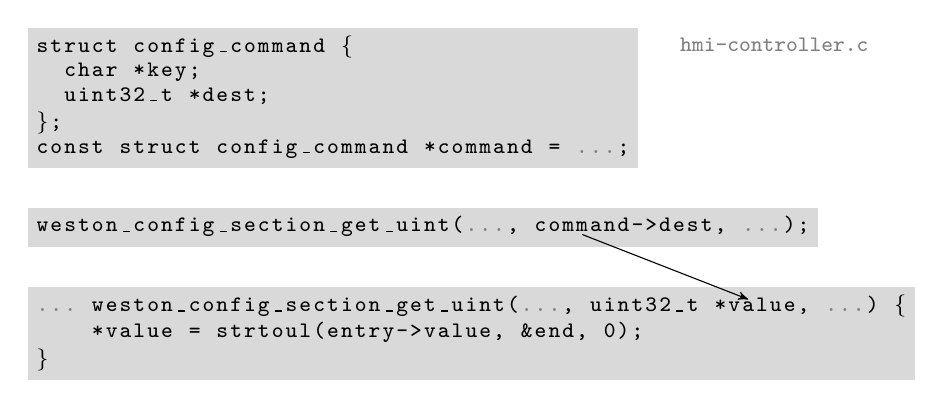
\begin{tikzpicture}
  [node distance=5mm, >=stealth',
  every node/.style={font=\footnotesize},
  every matrix/.style={fill=black!15, inner sep=1mm, row sep=0.5mm,
                        matrix of nodes, nodes in empty cells,
                        minimum height=0.5em, minimum width=.5em,
                        nodes={anchor=base, inner sep=0, font=\ttfamily\footnotesize}}]

  \matrix (command) {
s & t & r & u & c & t &   & c & o & n & f & i & g & \_ & c & o & m & m & a & n & d &   & \{ &   &   &   &   &   &   &   &   &   &   &   &   &   &   &   &   &   &   &   &   \\
  &   & c & h & a & r &   & * & k & e & y & ; &   &   &   &   &   &   &   &   &   &   &   &   &   &   &   &   &   &   &   &   &   &   &   &   &   &   &   &   &   &   &   \\
  &   & u & i & n & t & 3 & 2 & \_ & t &   & * & d & e & s & t & ; &   &   &   &   &   &   &   &   &   &   &   &   &   &   &   &   &   &   &   &   &   &   &   &   &   &   \\
\} & ; &   &   &   &   &   &   &   &   &   &   &   &   &   &   &   &   &   &   &   &   &   &   &   &   &   &   &   &   &   &   &   &   &   &   &   &   &   &   &   &   &   \\
c & o & n & s & t &   & s & t & r & u & c & t &   & c & o & n & f & i & g & \_ & c & o & m & m & a & n & d &   & * & c & o & m & m & a & n & d &   & = &   & |[black!50]|. & |[black!50]|. & |[black!50]|. & ; \\
  };

  \matrix [below=of command.south west, anchor=north west] (call) {
w & e & s & t & o & n & \_ & c & o & n & f & i & g & \_ & s & e & c & t & i & o & n & \_ & g & e & t & \_ & u & i & n & t & ( & |[black!50]|. & |[black!50]|. & |[black!50]|. & , &   & c & o & m & m & a & n & d & - & > & d & e & s & t & , &   & |[black!50]|. & |[black!50]|. & |[black!50]|. & ) & ; \\
  };

  \matrix [below=of call.south west, anchor=north west] (func) {
|[black!50]|. & |[black!50]|. & |[black!50]|. &   & w & e & s & t & o & n & \_ & c & o & n & f & i & g & \_ & s & e & c & t & i & o & n & \_ & g & e & t & \_ & u & i & n & t & ( & |[black!50]|. & |[black!50]|. & |[black!50]|. & , &   & u & i & n & t & 3 & 2 & \_ & t &   & * & v & a & l & u & e & , &   & |[black!50]|. & |[black!50]|. & |[black!50]|. & ) &   & \{ \\
  &   &   &   & * & v & a & l & u & e &   & = &   & s & t & r & t & o & u & l & ( & e & n & t & r & y & - & > & v & a & l & u & e & , &   & \& & e & n & d & , &   & 0 & ) & ; &   &   &   &   &   &   &   &   &   &   &   &   &   &   &   &   &   &   &   \\
\} &   &   &   &   &   &   &   &   &   &   &   &   &   &   &   &   &   &   &   &   &   &   &   &   &   &   &   &   &   &   &   &   &   &   &   &   &   &   &   &   &   &   &   &   &   &   &   &   &   &   &   &   &   &   &   &   &   &   &   &   &   &   \\
  };

  \node [above, anchor=west, black!50, xshift=0.5cm]
        at (command-1-43.north east)
        {\texttt{hmi-controller.c}};

  \draw [->] let \p1 = (call-1-40.south),
                 \p2 = (func-1-52.north)
              in (\p1) -- (\p2);

\end{tikzpicture}

\end{document}
